\chapter{Evaluation}
\label{sec:eval}
This chapter explains how we use the system described in \Cref{sec:approach} to evaluate its performance.
First, we review the results of the \ac{mcts} approach in \Cref{sec:eval:mcts}.
Next, we evaluate if we can use the results of the \ac{mcts} approach for learning to generate good schedules with supervised learning methods in \Cref{sec:eval:supervised}.
Lastly, we analyze and discuss the outcomes of the experiments in \Cref{sec:eval:discussion}.

\section{Hardware selection}
\label{sec:eval:hw}
There are different aspects in choosing the hardware for our experiments.
A processor must fulfill two aspects to be relevant for us.
The first is that LLVM supports it because we base our whole approach on LLVM and use the LLVM instruction scheduler as a baseline.
Secondly, we limit the hardware selection to processors that implement superscalar pipelines (see \Cref{sec:bg:superscalar-cpu}) because most modern processors implement these.

There are additional essential aspects regarding the hardware.
The most interesting one is if the processor implements an in-order superscalar pipeline or an out-of-order one.
While the former comes with no restrictions for our experiments, the latter can reschedule instructions during execution.
Followingly, it is interesting to see how the out-of-order model influences the performance of our approach.

Additionally, to show the versatility of our approach, it is interesting to choose different types of processors.
For example, there are classical \acp{cpu}, Edge \acp{cpu}, accelerator cards (\eg Graphical Processing Units (GPU), Vector Processing Units (VPU), and Intelligence Processing Units (IPU)).

With these aspects in mind, we select:
\begin{itemize}
    \item \textbf{AArch64 (Arm Cortex-A53):} This processor is an edge \ac{cpu} and implements an in-order superscalar pipeline based on the AArch64 architecture.
    An edge device that uses it is the Raspberry Pi 3 Model B.
    We use this device for our experiments with Ubuntu 20.04.
    \item \textbf{\aurora:} This processor is interesting because it implements an out-of-order superscalar pipeline. 
    Additionally, it is a vector processing accelerator card installed via a PCI-Express connection and thus a different type of processor.
\end{itemize}

\section{Monte Carlo Tree Search Schedule Search}
\label{sec:eval:mcts}
\begin{table}
    \centering
    \begin{tabular}{@{}lrr@{}}
        \toprule
        & \multicolumn{2}{c}{Processor} \\
        \cmidrule{2-3}
        MCTS Performance & AArch64 & \aurora \\
        \midrule
        \tblsection{Absolute} && \\
        \tblitem{Better than baseline}    & 54.79\% (7759) & 31.73\% (1349) \\
        \tblitem{Same as baseline}        & 36.97\% (5236) & 53.00\% (2253) \\
        \tblitem{Worse than baseline}     &  8.24\% (1167) & 15.27\%  (649) \\
        \tblsection{Runtime} && \\
        \tblitem{Mean Speed Up} & 8.35\% & 0.30\% \\
        \bottomrule
    \end{tabular}
    \caption[Results of the \ac{mcts} Approach]{Results of the \ac{mcts} approach. The \ac{mcts} approach was very successful on the AArch64 processor. We found better instruction schedules for more than the half of the basic blocks.
    On the \aurora, we are on par with the baseline for half of the basic blocks and fou nd better instruction schedules for a third of the basic blocks.}
    \label{tbl:eval:mcts}
\end{table}
% Goal of the experiment
We pursue two goals with this experiment.
One is to search instruction schedules that perform better than our baseline.
As our baseline, we choose the LLVM default instruction scheduler, implemented in the architecture-specific compiler back-end.
The second goal is to build a dataset that we can use for our supervised learning approaches.
As a side-effect, we will generate an upper limit for the supervised models.

% What do we do in this experiment
For each basic block under consideration, we first measure the runtime of the basic block compiled with the LLVM default instruction scheduler for the given processor.
Next, we generate an instruction schedule in each \ac{mcts} iteration.
We compile the instruction schedule into an executable format (\Cref{sec:approach:bbisolation}) and execute it to measure the runtime of the basic block of interest (\Cref{sec:approach:datageneration:runtime_methods}).
We train the \ac{mcts} model with the score computed by \Cref{eqn:approach:mcts-score} and start the next iteration to train the \ac{mcts} model.
This way, we generate many instruction schedules per basic block, each evaluated with a score based on their execution time relative to the default instruction schedule.

% Baseline

% How many (and which) BBs do we use
To have many instruction schedules available for our supervised learning methods, we select 20,032 basic blocks from the LLVM Test Suite.% \todo{describe how we got the basic blocks}
We generate one \ac{mcts} model for each basic block.
For this experiment, we have selected the longest basic blocks in the dataset.
The number of executions is not relevant in this experiment because we isolate the basic block and measure their specific runtime on the target hardware.
A high number of instructions in the basic blocks helps to avoid trivial scheduling situations.

% Number of steps to outroll the MCTS tree
The experiment is time-consuming because of the many basic blocks and the expensive compilation and runtime measurements.
We have to terminate the experiment at some point.
After 200 iterations, we have seen that we get a speedup for many basic blocks.
Therefore, we run the \ac{mcts} model for each basic block for 200 iterations.
The experiment execution took five weeks for the AArch64 processor, and three weeks for the \aurora.

% Exploration vs Exploitation balance weight
% WE DID NOT DESCRIBE THE FORMULAR NOWHERE

% Caching of schedules to detect duplicates
We try to avoid as many compilations and runtime measurements as possible because they take a long time.
Hence, we cache the generated schedules and reuse the measurements.
There are two caching levels in this approach:
First, we generate the instruction schedules in the format that the LLVM back-end uses and add the schedule to the cache.
The instruction schedule is then compiled to assembly code.
We cache the assemblies also because the format of the LLVM back-end still contains pseudo-instructions and can two different schedules can generate two equal assemblies.

% Performance: Summary of the excel tables
For the AArch64 we were able to run this experiment on 14,217 basic blocks.
Due to some errors, we measured an unrealistic speedup for some basic blocks.
Thus, we mark all speedup factors greater than two as outliers.
That leaves us with 14,162 valid instruction schedules for the AArch64 processor.
\Cref{tbl:eval:mcts} summarizes the results and shows that we find better-performing instruction schedules for 54.79\% of these basic blocks.
In only 8.24\% of the basic blocks, we did not find an instruction schedule that performed at least as well as the LLVM generated one.
On average, we increase the runtime performance of the basic blocks by 8.35\%.

We also executed this experiment for 4,253 basic blocks on the \aurora processor.
The lower number of basic blocks is caused by hardware and time limitations.
Only two outliers are generated during this experiment.%, which results in 4,251 valid basic blocks.
See \Cref{tbl:eval:mcts} for the summarized results.
For this processor, our \ac{mcts} approach found better instruction schedules for 31.73\% of the basic blocks.
In 15.27\% of the basic blocks, our model finds only worse instruction schedules.
The average speedup of the basic blocks is 0.30\%.

% In-order vs OoO discussion (Speed Up vs BB length)
If we run this experiment on more basic blocks, the results could still change in favor of the \aurora processor.
However, the observation that the performance on this processor is worse than on the AArch64 processor was expected.
The reason is that the \aurora is an out-of-order processor, and the AArch64 processor is an in-order processor.
That means, the \aurora might reschedule the instruction in hardware when it detects problems with the instruction schedule.
Thus, it does not depend on good instruction schedules as the AArch64 processor.

We showed with this experiment that we can find better instruction schedules for both our selected processors.
However, our search for instruction schedules was more successful for the AArch64 processor, as does no rescheduling in hardware.

\section{Supervised Schedule Generation}
\label{sec:eval:supervised}
As discussed, the \ac{mcts} approach is not usable for production systems because of its long runtime.
We use the dataset, generated by the \ac{mcts} approach, for other inference approaches in this section.
First, we evaluate the nearest-neighbor model and then the parametric models.

The dataset that we use for our supervised models is based on the results of the \ac{mcts} approach (\Cref{sec:eval:mcts}).
We split this dataset into a training set with 85\% randomly selected data points and a test set with the remaining 15\%.
\Cref{fig:eval:datasets} illustrates the usage of the created datasets.
\begin{figure}
    \centering
    \tikzstyle{defaultnode} = [text centered, align=center, font=\footnotesize\accentfont, rectangle, rounded corners, draw=black, minimum height=1cm, minimum width=2.5cm]
    \tikzstyle{arrow} = [thick,->,>=stealth,-{Latex[scale=1.2]}, font=\footnotesize\accentfont]
    \begin{tikzpicture}
        \node (bb)              [defaultnode] at ( 0,1) {Basic Blocks};
        \node (bbe)             [defaultnode] at ( 4.5,1) {Basic Blocks \\ + \\ Evaluated \\ Instruction Schedules};
        \node (training-set)    [defaultnode] at ( 8.5,2) {Training Set};
        \node (test-set)        [defaultnode] at ( 8.5,0) {Test Set};
        \node (model)           [defaultnode] at (13,2) {Supervised \\ Model};
        \node (eval)            [defaultnode] at (15.5,0) {Supervised \\ Evaluation};

        \draw [arrow] (bb) -- node [midway,above] {MCTS} (bbe);
        \draw [arrow] (bbe) |- node [midway,above] {85\%} (training-set);
        \draw [arrow] (bbe) |- node [midway,below] {15\%} (test-set);
        \draw (training-set) -- node [midway,above=0.4cm] {\footnotesize\accentfont Supervised} (model);
        \draw [arrow] (training-set) -- node [midway,above] {Training} (model);
        \draw [arrow] (test-set) -- node [midway,below] {Model Inference} (eval);
        \draw [arrow] (model) |- (eval);
    \end{tikzpicture}
    \caption[Overview over the used Dataset]{Overview over used datasets. The supervised model is one from \Cref{sec:eval:supervised}.}
    \label{fig:eval:datasets}
\end{figure}

These experiments aim to see if we can generate well-performing instruction schedules without auto-tuning methods, like the \ac{mcts} approach.

\subsection{Nearest Neighbor Model}
\begin{table}
    \centering
    \begin{tabular}{@{}lrr@{}}
        \toprule
        & \multicolumn{2}{c}{Processor}\\
        \cmidrule{2-3}
        Supervised Model & AArch64 & \aurora \\
        \midrule
        Nearest Neighbor & \textbf{1.38\%} & -3.03\% \\
        \tblsection{Support Vector Regression} && \\
        \tblitem{Balanced + Clustered} & -1.14\% & -3.53\% \\
        \tblitem{Balanced} & -1.18\% & -3.20\% \\
        \tblitem{Clustered} & -1.45\% & \textbf{-2.90\%} \\
        \tblsection{Neural Network} && \\
        \tblitem{Balanced + Clustered} & -0.48\% & -4.19\% \\
        \tblitem{Balanced} & -0.19\% & -3.19\% \\
        \tblitem{Clustered} & -0.47\% & -3.31\% \\
        \bottomrule
    \end{tabular}
    \caption[Performance of our Supervised Models]{Performance of our supervised models relative to the baseline:
    This table shows the mean speedup on the test set with our applied supervised learning models.
    Our nearest neighbor model performed best on the AArch64. 
    It is the only model that generated a positive mean speedup.
    On the \aurora, the SVR model with clustered instructions performed best.
    However, it is still worse than the baseline.}
    \label{tbl:eval:supervised-perf}
\end{table}

We use a large map structure to search our dataset for similar scheduling situations quickly.
\Cref{sec:app:nearest-neighbor} explains the details of this approach.
Then, we integrate this model into the LLVM compiler framework, and we use it to compile our basic blocks in the test set.

The instruction schedules that we compiled with this nearest-neighbor model for the AArch64 processor performed better than the baseline instruction scheduler from LLVM.
The measured runtimes for the basic block are 1.38\% shorter.
In fact, this is the only experiment where we exceeded the baseline performance with a supervised learning approach.
However, the measured runtimes on the \aurora processor are 3.03\% higher than the basic blocks compiled with the baseline instruction scheduler (see \Cref{tbl:eval:supervised-perf}).

\subsection{Parametric Machine Learning Models}
The parametric models require an additional data transformation to bring it into the form defined in \Cref{eqn:approach:regression-mapping}.
This results in a dataset of 4.9 million data points for the AArch64 architecture and 1.3 million data points for the \aurora architecture.
We add two variations to the parametric approaches, which we describe in the following paragraphs.
To see the effects of these variations, we run all approaches once with both and once with only one of the variations.

% \subsubsection{Instruction Clustering}
There are many similar instructions in the instruction sets of the two processors.
To reduce the dimensionality and simplify the dataset, we cluster some instructions into an alias instruction.
For example, we cluster the addition-instructions \lstinline|ADDWri| and \lstinline|ADDXri| of the AArch64 architecture into the same cluster.
These two instructions only differ in that one takes 32-bit values and the other 64-bit values.
See \Cref{appendix:instr-clusters} for exact clusterings.

% \subsubsection{Dataset Balancing}
Further, we balance our dataset in the target dimension, which holds the reward values from the \ac{mcts} trees.
The distribution of target values in our dataset roughly follows a normal distribution.
However, this can be problematic because the model might only learn to predict the mean of that distribution in any situation.
Therefore, we duplicate samples whose target value is further away from the mean and delete samples whose target value is very close to the mean.
% We sort the dataset into 40 histogram bins.
% In order to not distort the dataset too much, we delete at most 50\% of the samples in a histogram bin and do not increase the number of occurances of a sample to more than 30 times.
% \todo{How exactly}
This results in a dataset with a distribution closer to an equal distribution than to a normal distribution.
\begin{figure}
    \centering
    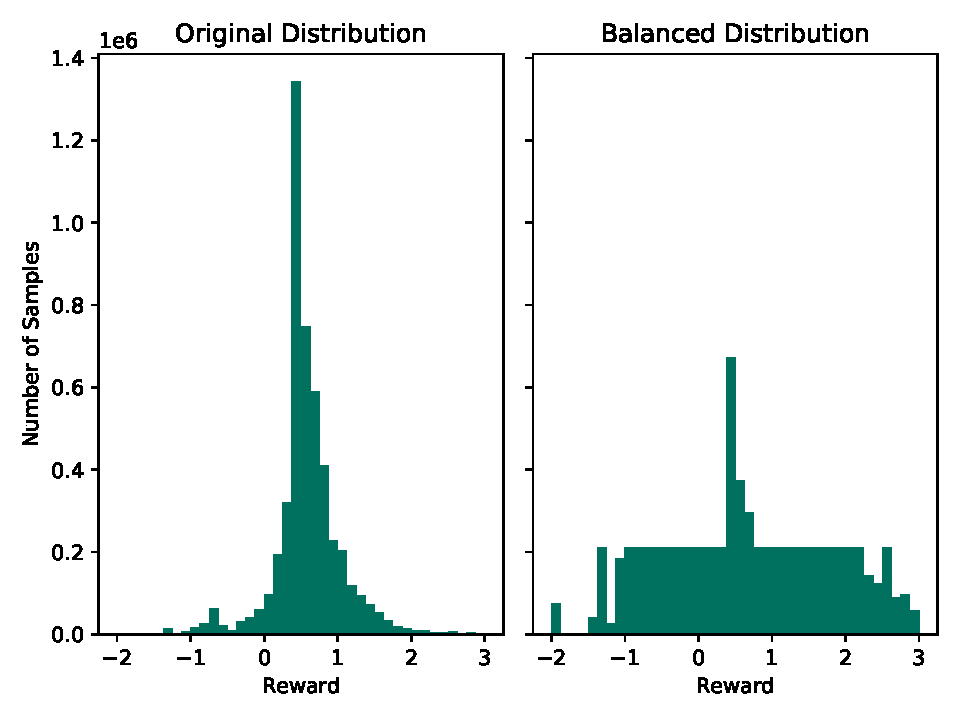
\includegraphics[width=0.75\textwidth]{img/balanced-supervised-dataset-rpi.pdf}
    \caption[Balancing for the AArch64 Dataset]{Balancing for the AArch64 dataset. 
    We duplicate samples with a reward further away from the distribution mean, and delete some samples that are close to the mean.}
    \label{fig:eval:balanced-dataset}
\end{figure}
\Cref{fig:eval:balanced-dataset} illustrates the effect on the distribution of the AArch64-dataset.
The effect for the \aurora dataset is similar.

\subsubsection{Support Vector Regression}
\label{sec:eval:svm}
\acp{svm} have long runtimes when trained with many data points.
We reduced this by randomly selecting 200,000 data points for the model training.

For the AArch64 processor, this model is the worst-performing one of the supervised learning models.
The measured runtimes of the scheduled basic blocks are 1.14\% to 1.45\% higher than the baseline's runtimes.

However, on the \aurora, we found this SVR approach combined with clustered instructions to be the best working parametric model.
Nevertheless, with a slowdown of 2.90\%, it still performs worse than on the AArch64 processor.

Regarding the effects of the dataset balancing and instruction clustering, we see no apparent effect.
For the AArch64 processor, the experiments with the balanced datasets perform better.
However, we observe the opposite effect for the \aurora.
Here, the dataset balancing negatively influenced the performance.

\subsubsection{Neural Network}
\label{sec:eval:nn}
For training the neural network, we use the early stopping scheme.
When the validation loss did not improve, for at least $10^{-6}$, once in the last ten epochs, we abort the training.
Computing the validation loss requires another split into training and validation set. 
We choose an 85/15 split again.

On the AArch64 processor, the scheduled basic blocks perform better than with the \ac{svr} approach.
With the balanced dataset, we get close to the baseline performance but we still perform worse than the baseline.

On the \aurora, the three neural network approaches performed the worst of all supervised learning approaches.
Here, the neural network approach with both, the balancing and clustering activated, is the worst of all approaches.


\section{Discussion}
\label{sec:eval:discussion}
\subsection{Applied History Length for Nearest Neighbor Approach}
\label{sec:eval:hist-length-vs-perf}
\begin{figure}
    \begin{subfigure}{\textwidth}
        \centering
        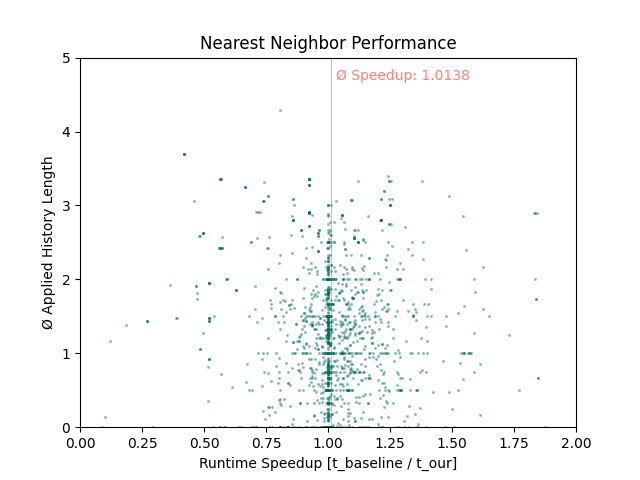
\includegraphics[width=0.75\textwidth]{img/nearest-neighbor/rpi_nn_scatter_no_outliers.png}
        \caption{AArch64}
        \label{fig:eval:nn-hist:pi}
    \end{subfigure}
    \vfill
    \begin{subfigure}{\textwidth}
        \centering
        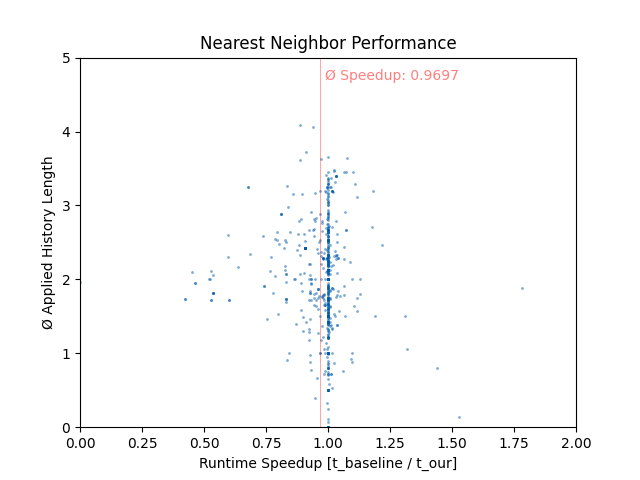
\includegraphics[width=0.75\textwidth]{img/nearest-neighbor/aurora_nn_scatter_no_outliers.png}
        \caption{\aurora}
        \label{fig:eval:nn-hist:aurora}
    \end{subfigure}
    \caption{Influence of the Applied History Length on Nearest Neighbor Speedup}
    \label{fig:eval:nn-hist}
\end{figure}
% What do we want to explain?
In order to understand the results of the nearest neighbor approach, we want to investigate the influence of the history length on the performance.
The history length is the number of previously scheduled instructions included when searching for relevant scheduling situations.
% Reminder of what applied history length means
We defined the maximum history length for our nearest neighbor model to be five instructions.
When searching for relevant scheduling situations, we might ignore some history instructions to find more relevant situations.
Therefore, we speak of an applied history length and take the average of the applied history lengths of all scheduling decisions in a basic block.
We refer to \Cref{sec:app:nearest-neighbor} for a detailed explanation.

% expected behaviour: more history -> better performance. Why is that expected?
Having a longer applied history length means that we make decisions based on more information.
Therefore, we expect that the runtime speedup is higher for basic blocks with a higher applied history length.
% Show if the expected behaviour is met, and why not
\Cref{fig:eval:nn-hist} illustrates each basic block in the test set with its runtime speedup and average applied history length.
However, we do not observe the expected correlation.
For the AArch64 processor, \Cref{fig:eval:nn-hist:pi} shows a big point cloud with no visible correlation.
\Cref{fig:eval:nn-hist:aurora} shows more worse-performing instruction schedules around an applied history length of 2 for the \aurora.
Still, there is no clear correlation observable.


\subsection{Effect of Partially Unknown Schedules in Monte Carlo Tree Search}
\label{sec:eval:unknown-schedules}
\begin{figure}
    \centering
    \begin{forest}
        [$h_n$
        [$\vdots$
        [$h_1$
        [$i_1$ [$?$[$?$[$\vdots$]] [$?$[$\vdots$]]] [$?$[$?$[$\vdots$]] [$?$[$\vdots$]]]]
        [$i_2$ [$?$[$?$[$\vdots$]] [$?$[$\vdots$]]] [$?$[$?$[$\vdots$]] [$?$[$\vdots$]]]]
        ]
        ]
        ]
    \end{forest}
    \caption[Nodes in the \ac{mcts} Tree that Influence the Rewards]{Nodes in the \ac{mcts} tree that influence the rewards:
    This scheduling situation has the history of instructions $h_1, \dots, h_n$ and the two candidate instructions $i_1$ and $i_2$.
    When either of the candidate instructions is selected, the schedule gets filled with randomly selected following candidate instructions.
    Thus, the score that the instructions $i_1$ and $i_2$ achieve do not depend only on itself and the history, but also on the randomly selected instructions.}
    \label{fig:eval:unknown-influence}
\end{figure}
The \ac{mcts} approach works well for searching well-performing instruction schedules for basic blocks.
However, the approaches that depend on the results of the \ac{mcts} did not reach comparable performances.
One reason for that might be the unknown latter part of the instruction schedules generated by \ac{mcts}.

As a reminder (see \Cref{sec:bg:mcts} for details): The \ac{mcts} approach starts with selecting instructions that already exist in its tree.
Once the algorithm reaches a leaf in a tree path, it selects random child nodes, \ie random candidate instructions.
Every node, \ie partial instruction schedule, has an assigned score.
However, this score depends not only on the partial instruction schedule already present in the tree but also on the following randomly selected instructions.
\Cref{fig:eval:unknown-influence} explains this with an example.

In tasks where nodes with similar rewards are grouped close together and nodes with differing rewards are further apart, that is no problem.
Contrarily, in our case, there seem to be single scheduling decisions that can significantly change the whole schedule's performance.
\Cref{fig:eval:changing-performance} illustrates an example of such a decision.
\begin{figure}
    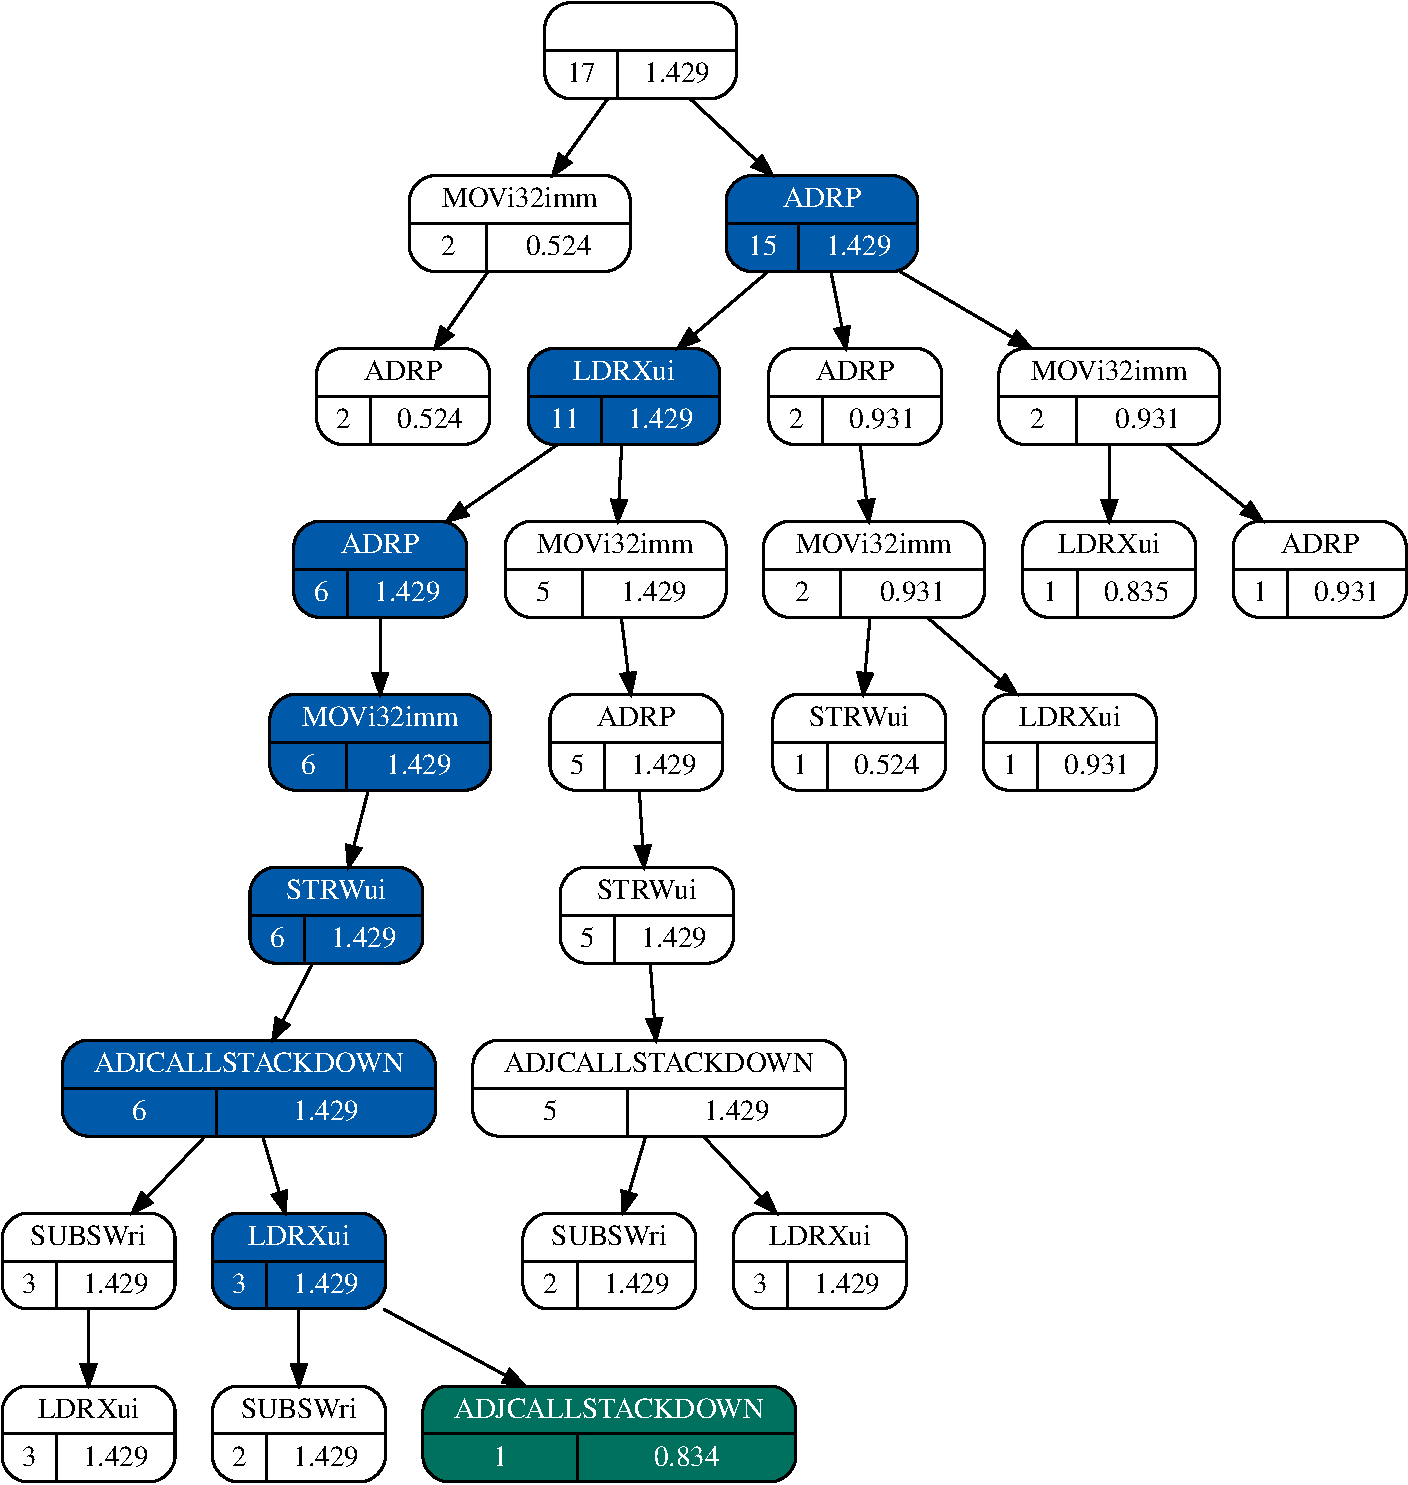
\includegraphics[width=\textwidth]{img/mcts-scores/2-crop.pdf}
    \caption[Importance of Single Scheduling Decisions]{Importance of Single Scheduling Decisions: All the blue partial paths have been evaluated with the score 1.429. 
    But after seven scheduling decisions, the deicision for the green instruction decreased the schedule performance to 0.834.
    This is an example from the \ac{mcts} approach for the AArch64 processor.}
    \label{fig:eval:changing-performance}
\end{figure}

As long as we use these random instructions only in the \ac{mcts} approach, it is no problem that they influence the rewards of partial schedules.
However, we use the tree also to generate the datasets that we use for the supervised learning approaches.
The problem is that we isolate scheduling decisions from its tree.
We use the previously scheduled instructions, the candidate instructions, and their score, but we do not have any information about the randomly selected instructions that also influence the score.
Therefore, the reliability of the rewards is limited.

The same problem applies analogously when we limit the history length and cut off instructions at the schedule's beginning.

\subsection{Conflicting Data in Regression Dataset}
There could be multiple reasons why the performance of the regression models cannot compete with the performance of the \ac{mcts} approach.
We investigate the number of conflicting data points in the dataset.
We consider two data points to be conflicting if they describe the same scheduling situation but have different rewards.
Conflicting data points can hurt the training process.
However, slight differences might be negligible.

\begin{figure}
    \centering
    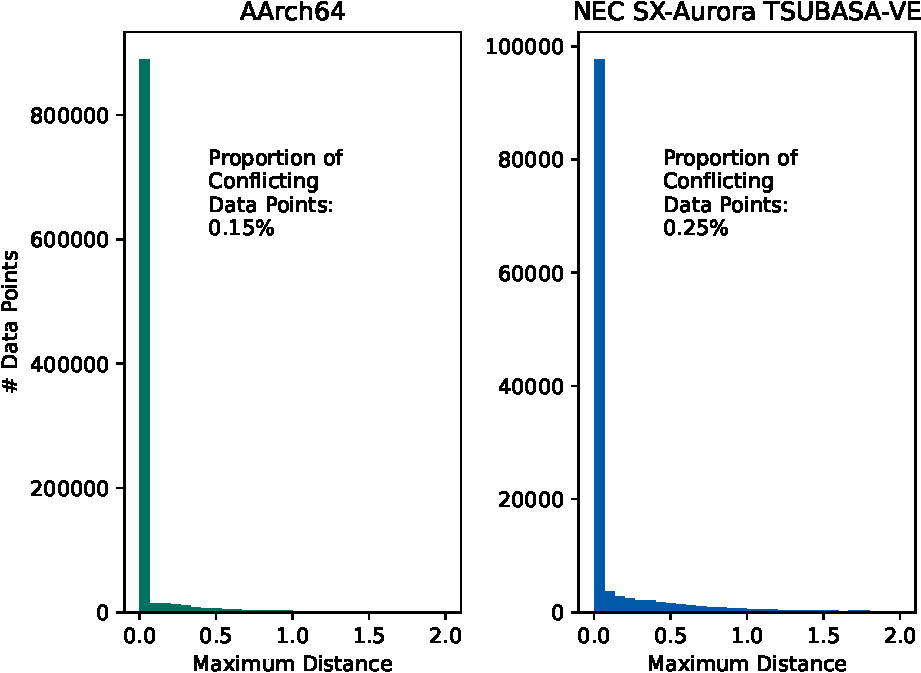
\includegraphics[width=0.8\textwidth]{img/hist-regr-conflicts-crop.pdf}
    \caption[Histogram Over the Maximum Difference Between Rewards of the Same Scheduling Situation]{Histogram Over the Maximum Difference Between Rewards of the Same Scheduling Situation:
    We see that for either architecture, there are conflicting data points.
    However, the number of conflicting data points is low.}
    \label{fig:eval:hist-conflicting-data-points}
\end{figure}
There might be multiple possible ways to find conflicting data points.
We compute the distance between the minimum and the maximum rewards for data points with the same scheduling situation.
\Cref{fig:eval:hist-conflicting-data-points} visualizes the distribution of these distances.
There are conflicting scheduling situations, but the large majority of data points is not conflicting.
Next, we could investigate the distribution of rewards for data points with the same scheduling situations.
However, this is not necessary because we have already seen, that the overall situation is acceptable.

Even though there are not many conflicting data points, it might still be worth it to clean the data.
The cleaning might be a difficult task because deciding which data points to prioritize is not trivial.
Note that this is one, but not the only, consequence of the problem from \Cref{sec:eval:unknown-schedules}.


\section{Summary}
The best supervised learning model that we have found is the nearest neighbor approach on the AArch64 processor.
In fact, it is the only one that performed better than the baseline instruction scheduler.
The neural network that was trained with the balanced dataset gets close to the baseline performance.

For the two dataset variations where we balanced the dataset and clustered similar instructions, we can see that the balancing was helping.
\Cref{tbl:eval:mcts} shows that the models trained with the balanced dataset performed better than with the clustered dataset in three out of four cases.
It even performed better than the approach with balanced and clustered dataset in three out of four cases.
In the other case it is close.
To summarise, the balancing helped overall, and the clustering had a negative influence on the performance.
It seems, that it indeed is important to differentiate between instructions that only differ in small aspects like the bit width. 

We have seen that our supervised approaches have all worked better on the AArch64 processor.
This was expected due to the smaller dataset and the low average speedup in the \ac{mcts} approach for the \aurora processor.
\Cref{tbl:eval:mcts} shows that the \aurora processor only achieved a 0.30\% speedup in the \ac{mcts} approach.
This value can be seen, as an upper limit for the supervised learning approaches because they are based on the results of the \ac{mcts} approach.

We observed that the applied history length does not have a clear influence on the performance of the nearest neighbor approach.
This requires additional investigation.
Additionally, we have discussed the expressiveness of \ac{mcts} rewards due to partial instruction schedules and their problematic effect on the dataset for supervised learning approaches.
Lastly, we showed a weakness of this dataset.
